\documentclass[a4paper,12pt]{article}
\usepackage[super,square]{natbib}		% Package to make citations superscrit with brackets
\usepackage{anysize}					% Package to change margin size
\marginsize{2cm}{2cm}{1cm}{2cm}
\usepackage{fancyhdr}					% Package to make headers
\renewcommand{\headrulewidth}{0pt}
\usepackage{soul}						% Package for highligths
\usepackage[dvipsnames]{xcolor}			% Colors for the references links
\usepackage{hyperref}					% Package to link references
\hypersetup{
    colorlinks=true,
    linkcolor=black,
    citecolor=CadetBlue,
    filecolor=CadetBlue,      
    urlcolor=CadetBlue,
}
\usepackage{lipsum}						% Package for lorem ipsum
\usepackage{multicol}					% Package for multicolumn
\setlength\columnsep{18pt}
\renewenvironment{abstract}				% Sets bastract
 {\par\noindent\textbf{Ringkasan}\ \ignorespaces \\}
 {\par\noindent\medskip}
% Change Contents and Reference
\renewcommand{\contentsname}{Daftar Isi}
\renewcommand\refname{Daftar Pustaka}

 
\begin{document}
% Makes header
\pagestyle{fancy}
\thispagestyle{empty}
\fancyhead[R]{\textit{Baltic Security Foundation}}
\fancyhead[L]{}
% Makes footnotes with an asterisk
\renewcommand*{\thefootnote}{\fnsymbol{footnote}}

\begin{center}
\Large{\textbf{\#1 Laporan Practice Big Data} -- \textit{Persiapan Environment}}
\vspace{0.4cm}
\normalsize \\ 
Nama mahasiswa (NIM) \\
Kelompok (Kelas) \\
\vspace{0.1cm}
\small{Prodi Teknologi Rekayasa Komputer Jaringan} \\
\small{Jurusan Teknologi Informasi dan Komputer} \\
\small{Politeknik Negeri Lhokseumawe}
\medskip
\normalsize
\end{center}

{\color{gray}\hrule}
\vspace{0.4cm}
\begin{abstract} 								% 5
\lipsum[1]
\end{abstract}
{\color{gray}\hrule}
\medskip
\begin{multicols}{2}
\tableofcontents
\section{Pendahuluan}
\lipsum[1]\cite{Bowker1985}

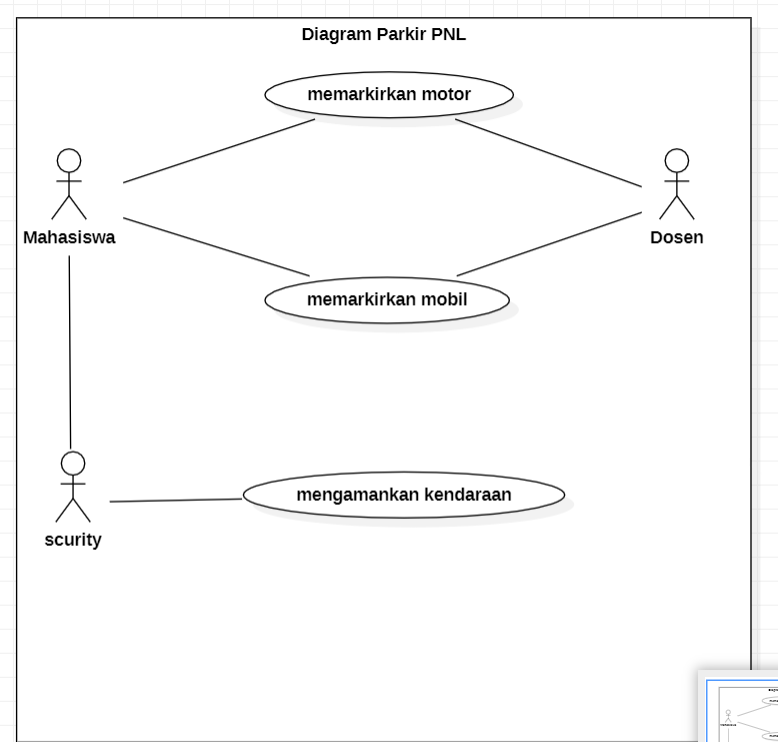
\includegraphics[scale=.5]{gambar/gambar1}

\subsection{Latar Belakang}
\lipsum[1]
\subsection{Tujuan}
\lipsum[1]
\subsection{Tinjauan Pustaka}
\lipsum[1]
\end{multicols}			% 15
{\color{gray}\hrule}
\begin{center}
\section{Alat dan Bahan}
\textbf{Sebutkan software dan hardware yang digunakan}
\end{center}
{\color{gray}\hrule}
\begin{multicols}{2}
\subsection{Alat}
Dalam praktikum instalasi Apache Hadoop, alat yang digunakan utamanya adalah personal komputer atau laptop. Berikut adalah jabaran rinci tentang penggunaan alat tersebut:

Personal Komputer atau Laptop:

Fungsi Utama: Alat ini digunakan sebagai pusat pengendalian dan pelaksanaan seluruh proses praktikum. Semua langkah-langkah instalasi dan konfigurasi dilakukan pada komputer atau laptop ini.
Sistem Operasi: Personal komputer atau laptop umumnya menjalankan sistem operasi Linux atau distribusi Linux tertentu seperti Ubuntu.
Spesifikasi Minimum: Disarankan untuk menggunakan komputer atau laptop dengan spesifikasi yang memadai untuk menjalankan Apache Hadoop. Hal ini termasuk kapasitas RAM yang cukup, ruang penyimpanan yang mencukupi, dan prosesor yang dapat menangani tugas-tugas yang diperlukan.

Akses Internet:

Fungsi Utama: Diperlukan koneksi internet untuk mengunduh perangkat lunak yang diperlukan selama praktikum, seperti OpenJDK, Apache Hadoop, dan paket-paket lainnya.
Proses Pengunduhan: Melibatkan penggunaan perintah seperti wget untuk mengunduh file Apache Hadoop dan apt untuk mengunduh dan menginstal paket-paket di Ubuntu.

Peralatan Input dan Output (Mouse, Keyboard, Monitor):

Fungsi Utama: Digunakan untuk interaksi langsung dengan komputer atau laptop selama proses instalasi dan konfigurasi. Keyboard dan mouse digunakan untuk memasukkan perintah, sedangkan monitor menampilkan hasil dan informasi yang diperlukan.

Terminal atau Command Line Interface (CLI):

Fungsi Utama: Sebagian besar langkah-langkah praktikum dilakukan melalui terminal atau command line interface. Pengguna akan memasukkan perintah-perintah untuk membuat grup, menginstal perangkat lunak, mengedit file konfigurasi, dan menjalankan perintah-perintah Hadoop.
Dengan menggunakan alat-alat tersebut, praktikan dapat secara langsung mengelola dan mengontrol proses instalasi dan konfigurasi Apache Hadoop pada lingkungan personal komputer atau laptop mereka.
\subsection{Bahan}
Untuk membuat praktikum perintah Hadoop menggunakan Virtual Box dan ISO Ubuntu, berikut adalah bahan-bahan yang umumnya digunakan:

Virtualization Software (Virtual Box):

Fungsi Utama: Digunakan untuk membuat dan mengelola mesin virtual.
Sumber: Dapat diunduh dan diinstal secara gratis dari situs resmi VirtualBox: https://www.virtualbox.org/

Image ISO Ubuntu:

Fungsi Utama: Diperlukan untuk menginstal sistem operasi Linux pada mesin virtual.
Sumber: Image ISO Ubuntu dapat diunduh dari situs resmi Ubuntu: https://ubuntu.com/download/desktop

Mesin Virtual:

Fungsi Utama: Dibuat menggunakan Virtual Box untuk menjalankan sistem operasi Ubuntu secara terisolasi.
Langkah-langkah:
Buat mesin virtual baru pada Virtual Box.
Atur parameter seperti jumlah RAM, kapasitas penyimpanan, dan jumlah prosesor.
Pilih image ISO Ubuntu yang telah diunduh sebagai media instalasi.

Koneksi Internet:

Fungsi Utama: Diperlukan untuk mengunduh paket dan perangkat lunak yang dibutuhkan selama instalasi dan konfigurasi.
Konfigurasi: Pastikan mesin virtual terhubung ke internet, baik melalui koneksi Wi-Fi atau kabel.

Terminal atau Command Line Interface (CLI):

Fungsi Utama: Digunakan untuk memasukkan perintah-perintah Hadoop dan menjalankan langkah-langkah praktikum.
Pada Ubuntu: Terminal dapat diakses langsung pada antarmuka grafis atau melalui pintasan keyboard (Ctrl + Alt + T).

Perangkat Lunak Apache Hadoop:

Fungsi Utama: Apache Hadoop perlu diunduh dan diinstal pada mesin virtual Ubuntu.
Sumber: Paket Apache Hadoop dapat diunduh dari situs resmi Apache Hadoop: https://hadoop.apache.org/
Dengan menggunakan kombinasi Virtual Box, ISO Ubuntu, dan perangkat lunak Apache Hadoop, Anda dapat membuat lingkungan virtual yang memungkinkan praktikan untuk belajar dan mengimplementasikan perintah-perintah Hadoop tanpa mempengaruhi sistem operasi utama pada komputer mereka.
\end{multicols}				% 20
{\color{gray}\hrule}
\begin{center}
\section{Prosedur Kerja}
\textbf{Jelaskan sesuai kondisi pada saat praktikum}
\end{center}
{\color{gray}\hrule}
\begin{multicols}{2}
\lipsum[1-2]
\end{multicols}


		% 25
{\color{gray}\hrule}
\begin{center}
\section{Hasil dan Pembahasan}
\textbf{Hasil dapat berupa gambar hasil praktikum, maupun data hasil praktikum}
\end{center}
{\color{gray}\hrule}
\begin{enumerate}

\item \textbf {Menjalankan Ubuntu dan Instalasi Hadoop}: \\ \\
    	\colorbox{BurntOrange}{wget https://dlcdn.apache.org/hadoop/common/hadoop-3.3.6/hadoop-3.3.6.tar.gz} \\ \\
    	
    	
\item \textbf {Beralih ke user hdoop}: \\ \\
\colorbox{BurntOrange}{su - hdoop} \\ \\
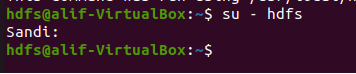
\includegraphics[scale=.6]{Gambar/satu} \\
    	
\item \textbf {Verifikasi Instalasi Java}: \\ \\
\colorbox{BurntOrange}{java -version} \\ \\
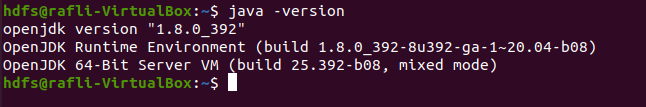
\includegraphics[scale=.6]{Gambar/dua} \\
    	
\item \textbf {Menjalankan Peintah-Perintah Hadoop}: \\ \\
\colorbox{BurntOrange}{start-dfs.sh} \\ \\
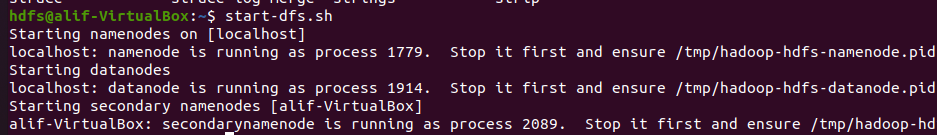
\includegraphics[scale=.5]{Gambar/tiga} \\
    	
\item \textbf {Verifikasi Hasil Instalasi Apache Spark}: \\ \\
\colorbox{BurntOrange}{pyspark --version} \\ \\
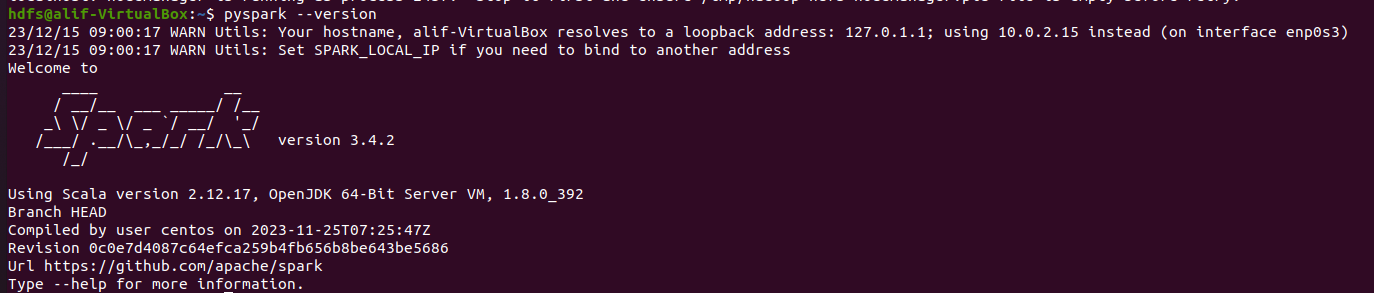
\includegraphics[scale=.4]{Gambar/empat} \\

\item \textbf {Menjalankan perintah jps}: \\ \\
\colorbox{BurntOrange}{jps} \\ \\
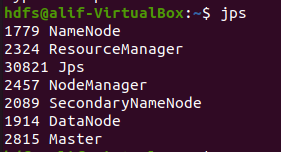
\includegraphics[scale=.4]{Gambar/lima} \\

\item \textbf {Menjalankan hadoop service di localhost}: \\ \\
\colorbox{BurntOrange}{Akses melalui web browser dengan alamat http://localhost: 98705 atau http://localhost:80886
.} \\ \\
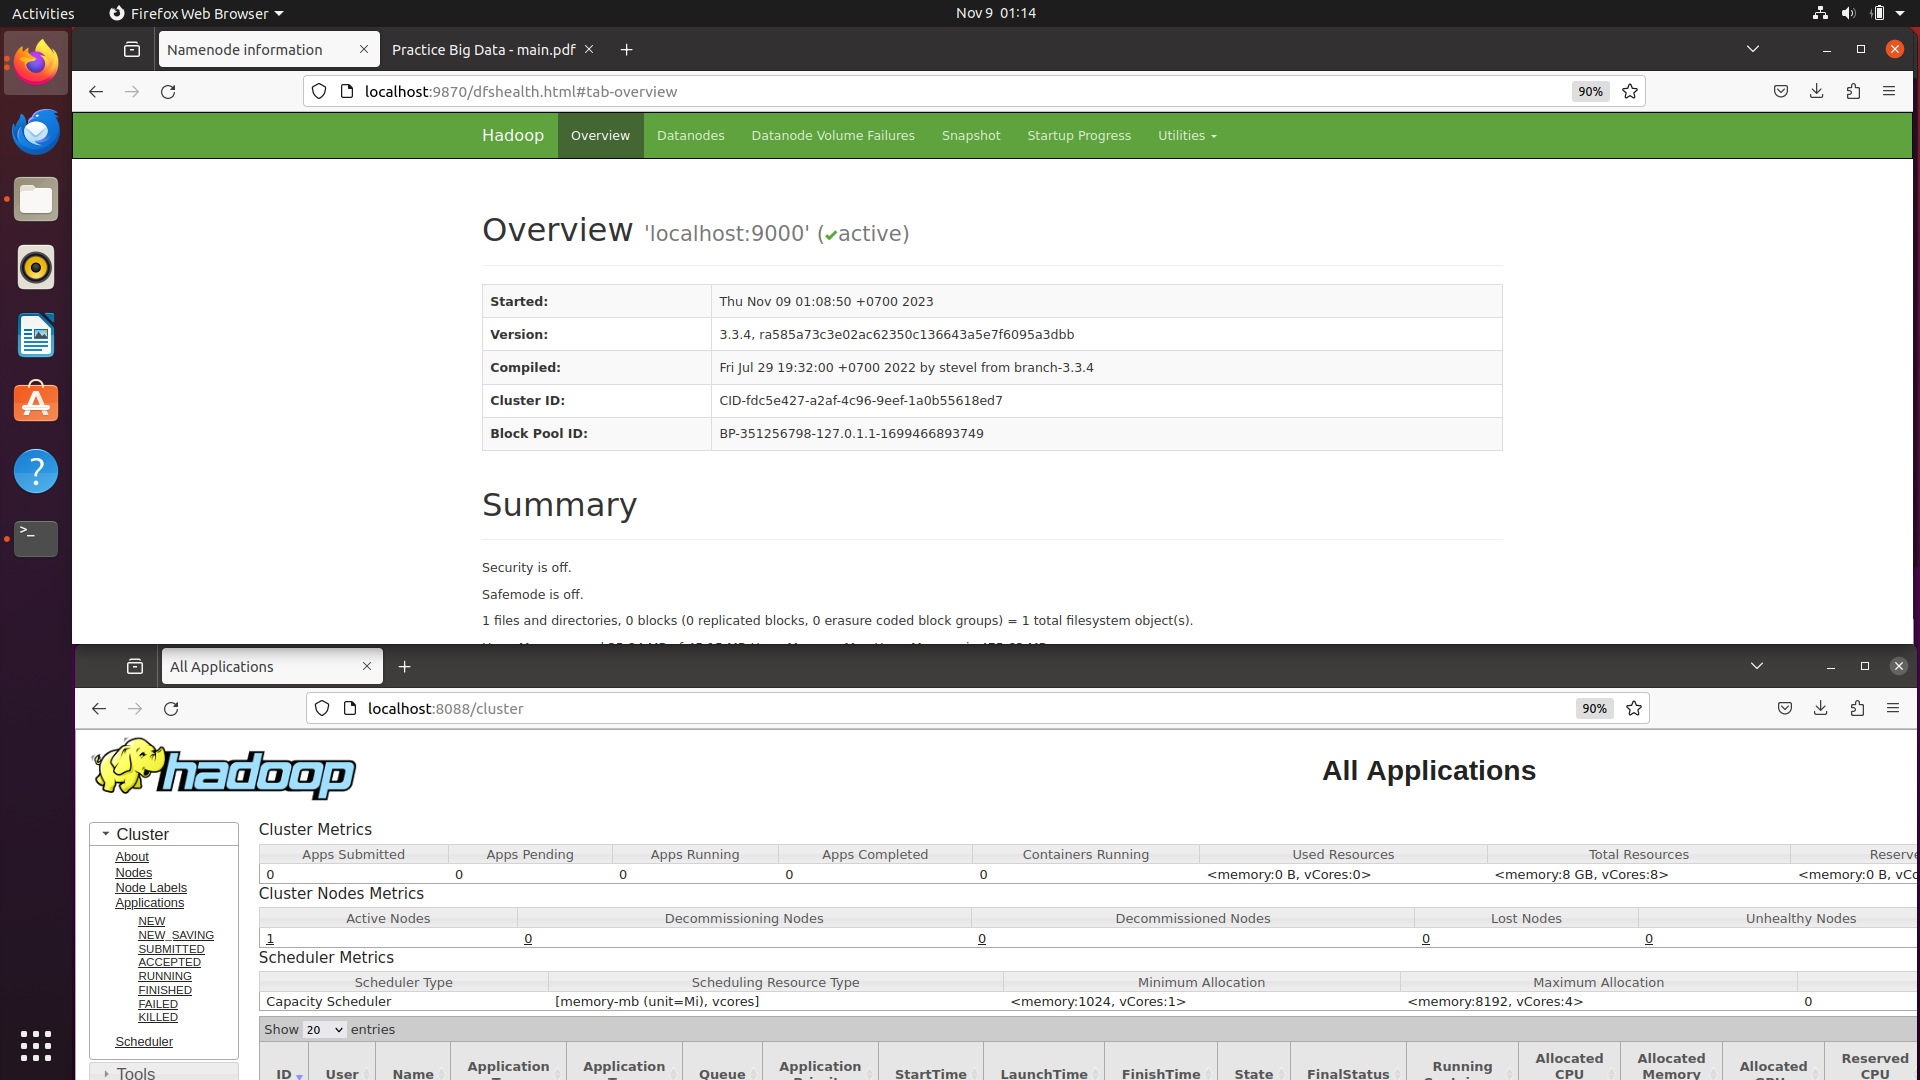
\includegraphics[scale=.2]{Gambar/hadoop sukses} \\

\item \textbf {Melihat hasil part 3}: \\ \\
\colorbox{BurntOrange}{hadoop fs -ls /output} \\ \\
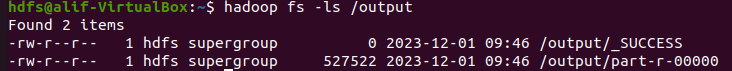
\includegraphics[scale=.4]{Gambar/enam} \\

\item \textbf {Melihat hasil grafik}: \\ \\
\colorbox{BurntOrange}{spark - submit MLPySpark.py} \\ \\
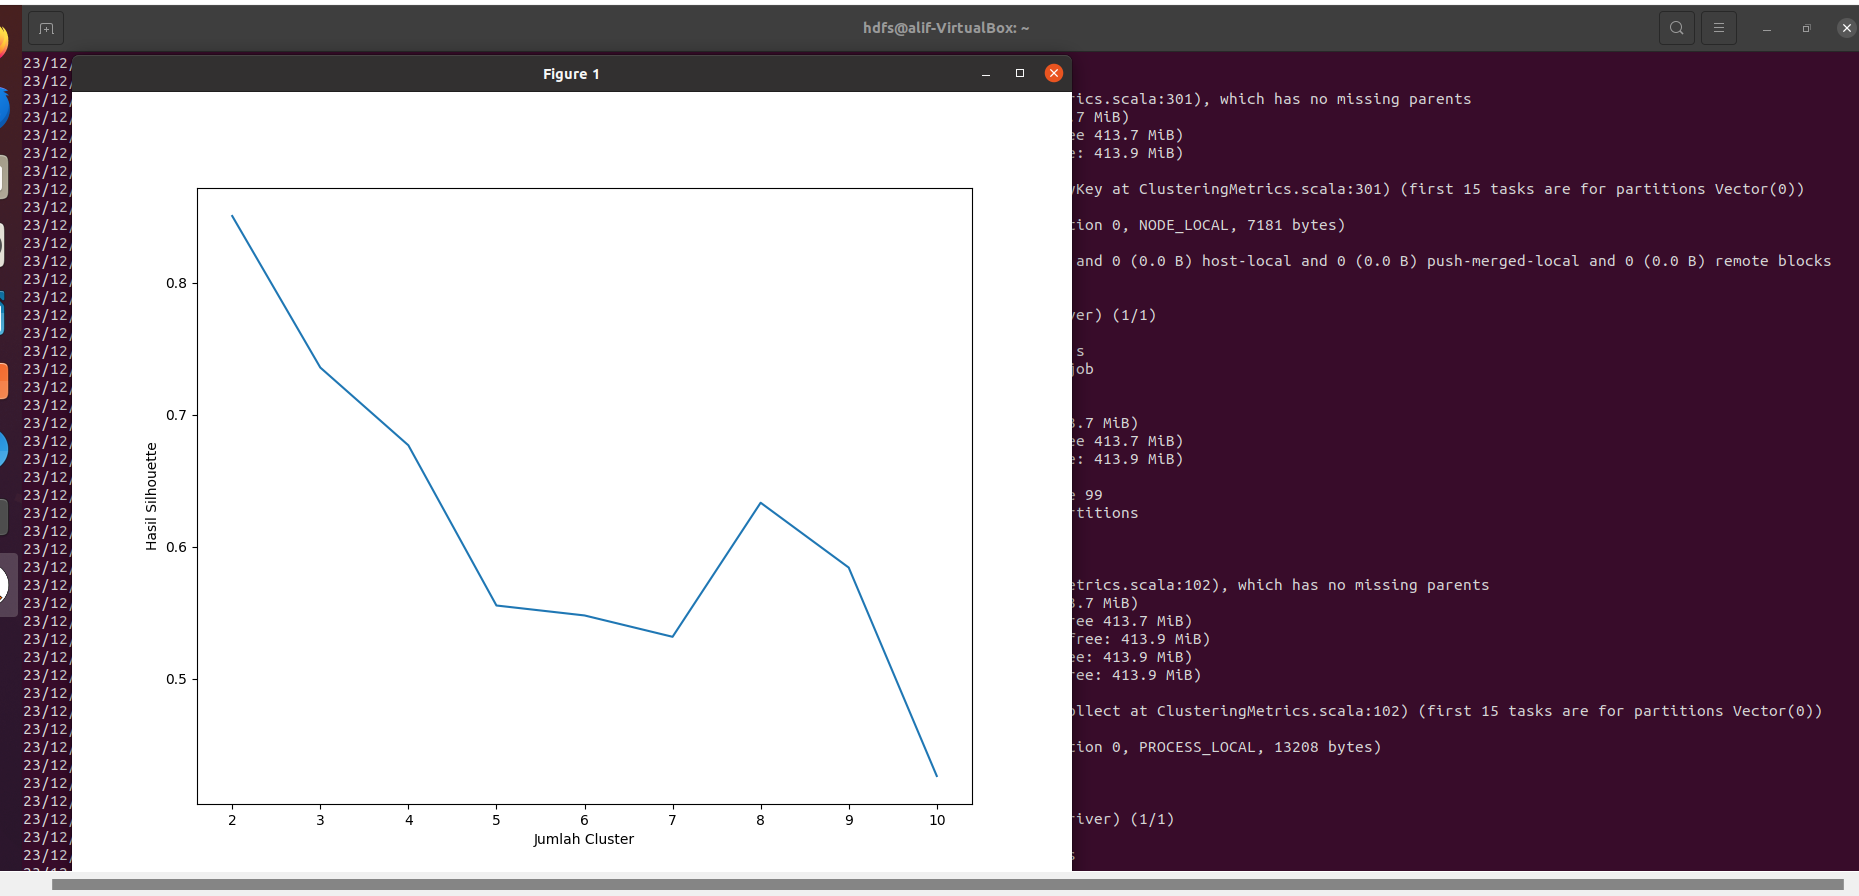
\includegraphics[scale=.4]{Gambar/tujuh} \\



    	
    	
 
    	
    	 	
    	
    	
    	
    	
    	
    	
    	
    	
    	
    	
    	
    	
    	
    	
    	
    	
    	
    	
    	
    	
    	
    	
    	
    	
    	
    	
    	
    	
    	
    	
    	
    	
    	
    	
    	
    	
    	
    	
    	
    	
    	
    	
    	
    	
    	
    	
    	
    	
    	
    	
    	
    	
    	
    	
    	
    	
    	
    	
    	
    	
    	
    	
    	
    	
    	
    	
    	
    	
    	
\end{enumerate}

		% 25
{\color{gray}\hrule}
\begin{center}
\section{Kesimpulan}
\textbf{Uraikan kesimpulan hasil praktikum}
\end{center}
{\color{gray}\hrule}
\vspace{0.5cm}
\lipsum[1]				%  5
\bibliographystyle{plain}
\bibliography{references}						%  5 - minimal terdapat 2 daftar pustaka
\end{document}